\documentclass{ceurart}
\sloppy
\usepackage{listings}
\lstset{breaklines=true, keywordstyle=\bfseries}
\usepackage[inline]{enumitem}
\usepackage{tikz}
\usetikzlibrary{decorations.pathreplacing}
\usepackage{caption}
\usepackage{subcaption}

\begin{document}

\copyrightyear{2024}
\copyrightclause{Copyright for this paper by its authors. Use permitted under Creative Commons License Attribution 4.0 International (CC BY 4.0).}
\conference{ITADATA 2024 - BigHPC, Pisa, Italy - 17-19 September 2024}
\title{Quantum-Classical Sentiment Analysis}
\author[1]{Mario Bifulco}[email=mario.bifulco@edu.unito.it,url=https://github.com/TheFlonet/qsvm4sentanalysis]
\author[1]{Luca Roversi}[orcid=0000-0002-1871-6109,email=luca.roversi@unito.it,url=https://www.di.unito.it/~rover/]
\address[1]{Università degli studi di Torino, Dipartimento di Informatica, Corso Svizzera 185 - 10149 Torino}

\begin{abstract}
    In this work, we first experiment with applying a hybrid classical-quantum classifier (HCQC) for sentiment analysis and compare it to the classical CPLEX classifier and Transformer architecture. We find that HCQC is worse than Transformer in classification, but takes much less time to converge to a reasonably good approximate solution. Secondly, the work explores how to address what we may consider a bottleneck of HCQC, whose architecture is partially undisclosed by the D-Wave property. The results show how effective hybrid solvers can be developed to avoid the opaque systems proposed by D-Wave, thus making greater use of the quantum component.
\end{abstract}
\begin{keywords}
    Quantum Adiabatic Computing \sep 
    Machine Learning \sep
    Sentiment Analysis \sep 
    Hybrid solver 
\end{keywords}

\maketitle

\section{Introduction}
In natural language processing, the two main challenges in developing new models are the difficulty in acquiring high-quality data and the extensive training times required to make models more expressive\cite{scaling}.

This work focuses on the latter issue. We experiment with unconventional computing architectures, the goal being to assess if and how they can help accelerate training time to obtain more expressive models. To this purpose, our choice is architectures that develop Adiabatic Quantum Computing (AQC), where the technology proposed by D-Wave is considered a standard. The reason is twofold. On one side AQC by its very nature solves minimization problems in the QUBO form (Quadratic Unconstrained Binary Optimization). On the other, the core of many AI problems is minimizing some functions by looking for the values of specific parameters.

We choose SVM\cite{SVM} over more standard Transformers models because preliminary investigations on SVMs that leverage AQC already exist\cite{QSVM} and SVM share some similarities with the attention mechanism of Transformers\cite{TransformerSVM}.

Precalling that, among classification tasks in natural language processing, the binary version of Sentiment Analysis (BSA) aims to separate sentences that convey ``positive'' emotions from those that convey ``negative'' emotions. We reduced the BSA to QUBO and evaluated the following:
\begin{enumerate*}[label=\arabic*)]
    \item performance during classification;
    \item the time required to train the model;
    \item the time required to classify new examples,
\end{enumerate*}
compared to more standard techniques implemented with heuristics and classical architectures. To improve our results relative to training time we also started to investigate software-based alternatives to the proprietary mechanisms that physically embed QUBO problems on Quantum CPU (QPU) for AQC. We shall briefly report on this in the conclusion.

\section{Quantum Support Vector Machine for Sentiment Analysis}

We choose TweetEval\cite{TweetEval} to verify the effectiveness of SVM for BSA. TweetEval is considered a standard for comparing different models and contains a sufficiently large and representative number of examples, i.e. Tweets extracted from \url{https://x.com/} and labelled automatically. The ``sentiment'' split of TweetEval includes three classes: positive, negative and neutral. We choose to discard all ``neutral'' samples to avoid introducing errors during learning due to examples belonging to non-expressive classes. Additionally, we normalize the quantity of elements in the positive and negative classes to ensure a balanced dataset.

Since SVMs do not natively support text processing, it is necessary to compute embeddings. Among the various possibilities, SentenceBert\cite{SentenceBert} allows for capturing the contextual information of the entire sentence by producing a single embedding.

For comparison with the classical counterpart, we choose:
\begin{enumerate*}[label=\arabic*)]
    \item the CPLEX\cite{cplex} solver, a widely used optimizer for solving both linear and non-linear programming problems;
    \item RoBERTa\cite{ROBERTA}, a deep-learning model based on BERT\cite{BERT} and the attention mechanism\cite{Attention}.
\end{enumerate*}
RoBERTa allows a fair comparison as the model we use\cite{robertamodel} is fine-tuned on TweetEval.

\begin{table}
    \caption{Classification results}
    \label{tab:classification}
    \begin{tabular}{cccc}
        \toprule
        & D-Wave & CPLEX & RoBERTa \\
        \midrule
        F1-Score (\%) & 76.1 & 76.9 & 94.3 \\
        Train time (s) & 39.2 & 101.9 & / \\
        Eval time (s) & 33.9 & 2.2 & 136.8 \\
        \bottomrule
    \end{tabular}
\end{table}

Table \ref{tab:classification} shows some data related to the training and inference of the different models compared. D-Wave stands for what we develop in this work and report on here.

\paragraph{F1 score} The classification conducted by RoBERTa is significantly better, although the results of both CPLEX and D-Wave are also well above random guesses. The slight difference between the solution obtained with CPLEX and that with D-Wave may be due to some limitations of the current hybrid solvers, which restricted the domain of the optimisation variables from real numbers to integers.

\paragraph{Training time} The time required by D-Wave to find an optimal assignment is 60\% less than that of the classical counterpart. Although not available, it is reasonable to expect an even better result if compared to the time required by RoBERTa, which we can fairly expect to amount to several hours of training on high-performance machines.

\paragraph{Prediction time} The complexity of RoBERTa architecture also affects the time required for prediction by requiring more computing time than CPLEX or D-Wave. The higher time required is due to D-Wave returning a set of optimal solutions. For each of them, a model is created to apply a majority vote to establish the class in inference. Since no advantages emerge from using several models, it is possible to use only one of the optimal assignments, reducing the time to values comparable to those of CPLEX.

\section{Maximizing quantum boost}

Using the \emph{default} hybrid solver by D-Wave entails an opaque workflow due to the underlying proprietary technology. Examination of the available data, however, shows that to obtain the values in Table \ref{tab:classification} the QPU contributes very marginally, averaging 0.08\%. Since the performance boost should derive from the quantum component, it is worth considering whether it is possible to use a greater amount of it, ideally shifting the entire problem resolution onto the QPU and delegating only pre- and post-processing operations to some CPUs or GPUs.

Direct access to the QPU is possible provided you manually perform certain pre-processing operations of the problem such as:
\begin{enumerate}
    \item Convert the problem into QUBO form i.e:
    \begin{enumerate*}
        \item to incorporate the constraints into the objective as penalty functions via appropriately parameterised Lagrangian relaxation\cite{QbridgeI};
        \item to convert the optimisation variables into binary variables;
        \item to transform the objective function into a minimisation problem.
    \end{enumerate*}
    \item Search for the minor\cite{ME}\cite{MEdwave} associated with the QUBO problem that can be mapped onto the D-Wave QPU's physical graph architecture, Figure \ref{fig:pegasus}.
\end{enumerate}

By performing these steps independently, it is possible to bypass D-Wave's proprietary technology to try to maximise QPU usage. The only operation with high computational cost among those described is the search for the minor embedding, which is NP-complete. For this reason, Table \ref{tab:embedding} focuses on the time required to compute the minor embedding of the graph representing an SVM. We can see that, for 128 variables, the calculation takes more than 7 minutes and occupies about 38\% of the 5600 qubits available on the QPU. This makes the direct use of the QPU not applicable to real-size problems.

\begin{table}
    \caption{Embedding search time}
    \label{tab:embedding}
    \begin{tabular}{ccccccc}
        \toprule
        Problem nodes & 4 & 8 & 16 & 32 & 64 & 128 \\  
        \midrule
        Embedding Nodes & 4 & 13 & 40 & 138 & 526 & 2117 \\
        Avg Time (s) & 0.2 & 0.3 & 0.6 & 6.1 & 53.4 & 434.2 \\
        \bottomrule
    \end{tabular}
\end{table}

\section{Homebrewing a Hybrid Solver}

Given the practical impossibility of using the QPU directly, it is unavoidable to rely on hybrid solvers. Therefore, we investigate how to design a hybrid solver, called \verb|QSplit|, to increase the use of the QPU, based on a quite simple algebraic technique that decomposes QUBO problems into smaller chunks. Sufficiently small problems can be solved by mapping them on the QPU, eventually aggregating the results. This technique is of general application, not limited to QUBO instances we get from SVM.

\begin{figure}
    \centering
    \begin{subfigure}[c]{0.54\textwidth}
        \centering
        \resizebox{0.54\textwidth}{!}{%
            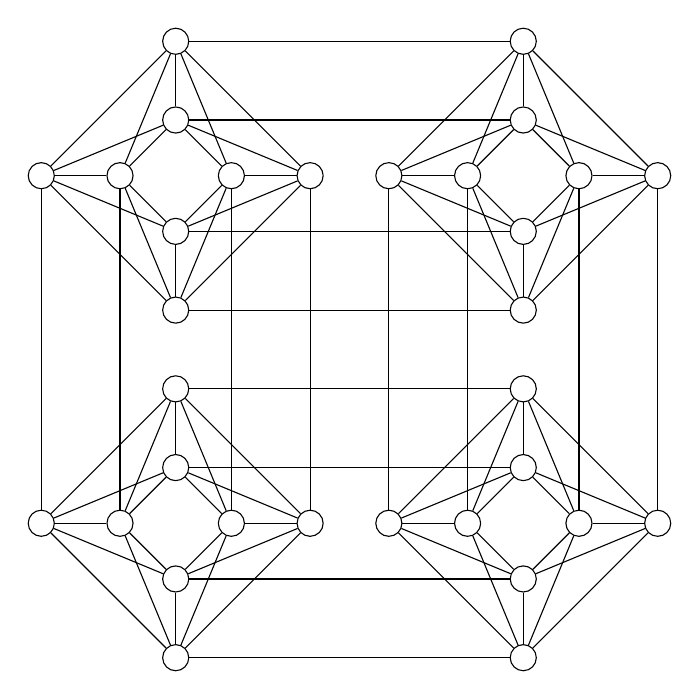
\begin{tikzpicture}[main/.style = {draw, circle}] 
                \node[main](1){};
                \node[main](2)[right of=1]{}; 
                \node[main](5)[above right of=2]{};
                \node[main](6)[above of=5]{};
                \node[main](3)[below right of=5]{};
                \node[main](4)[right of=3]{};
                \node[main](7)[below right of=2]{};
                \node[main](8)[below of=7]{};
        
                \draw (1) -- (6);\draw (6) -- (4);\draw (4) -- (8);\draw (8) -- (1);
                \draw (1) -- (5);\draw (5) -- (4);\draw (4) -- (7);\draw (7) -- (1);
                \draw (6) -- (2);\draw (2) -- (8);\draw (8) -- (3);\draw (3) -- (6);
                \draw (2) -- (5);\draw (5) -- (3);\draw (3) -- (7);\draw (7) -- (2);
                \draw (1) -- (2);\draw (5) -- (6);\draw (3) -- (4);\draw (8) -- (7);
        
                \node[main](11)[right of=4]{};
                \node[main](12)[right of=11]{}; 
                \node[main](15)[above right of=12]{};
                \node[main](16)[above of=15]{};
                \node[main](13)[below right of=15]{};
                \node[main](14)[right of=13]{};
                \node[main](17)[below right of=12]{};
                \node[main](18)[below of=17]{};
        
                \draw (11) -- (16);\draw (16) -- (14);\draw (14) -- (18);\draw (18) -- (11);
                \draw (11) -- (15);\draw (15) -- (14);\draw (14) -- (17);\draw (17) -- (11);
                \draw (16) -- (12);\draw (12) -- (18);\draw (18) -- (13);\draw (13) -- (16);
                \draw (12) -- (15);\draw (15) -- (13);\draw (13) -- (17);\draw (17) -- (12);
                \draw (11) -- (12);\draw (15) -- (16);\draw (13) -- (14);\draw (18) -- (17);
        
                \node[main](26)[below of=8]{};
                \node[main](25)[below of=26]{};
                \node[main](22)[below left of=25]{};
                \node[main](21)[left of=22]{};
                \node[main](23)[below right of=25]{};
                \node[main](24)[right of=23]{};
                \node[main](27)[below right of=22]{};
                \node[main](28)[below of=27]{};
        
                \draw (21) -- (26);\draw (26) -- (24);\draw (24) -- (28);\draw (28) -- (21);
                \draw (21) -- (25);\draw (25) -- (24);\draw (24) -- (27);\draw (27) -- (21);
                \draw (26) -- (22);\draw (22) -- (28);\draw (28) -- (23);\draw (23) -- (26);
                \draw (22) -- (25);\draw (25) -- (23);\draw (23) -- (27);\draw (27) -- (22);
                \draw (21) -- (22);\draw (25) -- (26);\draw (23) -- (24);\draw (28) -- (27);
        
                \node[main](36)[below of=18]{};
                \node[main](35)[below of=36]{};
                \node[main](32)[below left of=35]{};
                \node[main](31)[left of=32]{};
                \node[main](33)[below right of=35]{};
                \node[main](34)[right of=33]{};
                \node[main](37)[below right of=32]{};
                \node[main](38)[below of=37]{};
        
                \draw (31) -- (36);\draw (36) -- (34);\draw (34) -- (38);\draw (38) -- (31);
                \draw (31) -- (35);\draw (35) -- (34);\draw (34) -- (37);\draw (37) -- (31);
                \draw (36) -- (32);\draw (32) -- (38);\draw (38) -- (33);\draw (33) -- (36);
                \draw (32) -- (35);\draw (35) -- (33);\draw (33) -- (37);\draw (37) -- (32);
                \draw (31) -- (32);\draw (35) -- (36);\draw (33) -- (34);\draw (38) -- (37);
        
                \draw (6) -- (16);
                \draw (5) -- (15);
                \draw (7) -- (17);
                \draw (8) -- (18);
                \draw (26) -- (36);
                \draw (25) -- (35);
                \draw (27) -- (37);
                \draw (28) -- (38);
                \draw (1) -- (21);
                \draw (2) -- (22);
                \draw (3) -- (23);
                \draw (4) -- (24);
                \draw (11) -- (31);
                \draw (12) -- (32);
                \draw (13) -- (33);
                \draw (14) -- (34);
            \end{tikzpicture} 
        }  
        \caption{Example of 32 qubit QPU\cite{Pegasus}}
        \label{fig:pegasus}
    \end{subfigure}
    \hfill
    \begin{subfigure}[c]{0.45\textwidth}
        \centering
        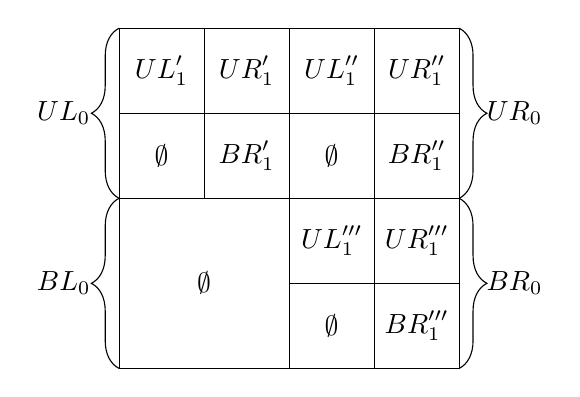
\begin{tikzpicture}[scale=0.54]
            \draw (0,0) rectangle (8,8);
        
            \draw (0,4) -- (8,4);
            \draw (4,0) -- (4,8);
            \node at (2,2) {$\emptyset$};
            
            \draw (0,6) -- (4,6);
            \draw (2,8) -- (2,4);
            \node at (1,5) {$\emptyset$};
        
            \draw (4,2) -- (8,2);
            \draw (6,4) -- (6,0);
            \node at (5,1) {$\emptyset$};
    
            \draw (4,6) -- (8,6);
            \draw (6,4) -- (6,8);
            \node at (5,5) {$\emptyset$};
        
            \draw[decorate,decoration={brace,amplitude=10pt}] (8,8) -- (8,4) node [black,midway,xshift=20pt] {$\operatorname{UR}_0$};
            \node at (3,7) {$\operatorname{UR}_1'$};
            \node at (7,7) {$\operatorname{UR}_1''$};
            \node at (7,3) {$\operatorname{UR}_1'''$};
    
            \draw[decorate,decoration={brace,amplitude=10pt,mirror}] (0,8) -- (0,4) node [black,midway,xshift=-20pt] {$\operatorname{UL}_0$};
            \node at (1,7) {$\operatorname{UL}_1'$};
            \node at (5,7) {$\operatorname{UL}_1''$};
            \node at (5,3) {$\operatorname{UL}_1'''$};
    
            \draw[decorate,decoration={brace,amplitude=10pt}] (8,4) -- (8,0) node [black,midway,xshift=20pt] {$\operatorname{BR}_0$};
            \node at (3,5) {$\operatorname{BR}_1'$};
            \node at (7,5) {$\operatorname{BR}_1''$};
            \node at (7,1) {$\operatorname{BR}_1'''$};

            \draw[decorate,decoration={brace,amplitude=10pt,mirror}] (0,4) -- (0,0) node [black,midway,xshift=-20pt] {$\operatorname{BL}_0$};
        \end{tikzpicture}
        \caption{Two steps of recursive decomposition}
        \label{fig:qubo}
    \end{subfigure}
    \caption{QPU graph structure (\ref{fig:pegasus}) and decomposition of QUBO matrix (\ref{fig:qubo})}
\end{figure}

Given any QUBO matrix we recursively divide it into four parts as in Figure \ref{fig:qubo}:
\begin{enumerate*}[label=\arabic*)]
    \item $\operatorname{ULs}$ and $\operatorname{BRs}$ are themselves QUBO matrices operating on a partition of the optimization variables;
    \item $\operatorname{UR}$ is not guaranteed to be upper triangular, as required by a QUBO instance, but it retains the information linking the partitions $\operatorname{UL}_0$, $\operatorname{BL}_0$ and $\operatorname{UR}_0$, $\operatorname{BR}_0$ of the variables and we can safely transform it into an upper triangular matrix, namely a QUBO instance;
    \item $\emptyset$ is a matrix composed entirely of zeros, so we ignore it.
\end{enumerate*}

The recursive subdivision can continue until the matrices reach a predetermined size. Compatible with the results of Table \ref{tab:embedding}, directly solving $32 \times 32$ matrices via QPU might be a good compromise for using \verb|QSplit| in real-world contexts.

Let us see how an inductive step of the process works. Let us assume that we have classifications offered by $\operatorname{UL}_1'$, $\operatorname{UR}_1'$, $\operatorname{BR}_1'$. The classification offered by:
\begin{enumerate*}[label=\arabic*)]
    \item $\operatorname{UL}_1'$ and $\operatorname{BR}_1'$ can be combined to generate conflict-free initial assignments called $\operatorname{S_1}$;
    \item $\operatorname{UR}_1'$ offers classifications based on two partitions of variables. In practice, it is solved by incorporating the coefficients of a matrix of zeros of size $\operatorname{UL}_0$. Although this could lead to matrices larger than the bounds tested in Table \ref{tab:embedding}, its graph structure is small enough to allow for manageable computation times directly on the QPU.
\end{enumerate*}
The solutions from $\operatorname{S_1}$ and those obtained from $\operatorname{UR}_1'$ are combined by searching for compatible assignments and marking conflicting variables. From the conflicting values, a QUBO problem is extracted, considering only the rows and columns associated with these variables, which is again solved via QPU. Of course, the proposed method of resolving conflicting assignments could, in the worst case, require reconsideration of the entire problem \(\operatorname{UL}_0\), nullifying the decomposition process and leading to intractable cases. However, the problem did not show up in our tests. From the set of possible assignments obtained by solving conflicting classifications, duplicates are removed and only the $k$ most promising assignments are retained. This is a heuristic that should help avoid an exponential increase in the number of solutions to be aggregated.

\begin{table}
    \centering
    \begin{tabular}{cccccc}
        \toprule
        Stop dim & Time (s) & Proposed solution & Direct time (s) & Direct solution & Estimated range \\
        \midrule
        2 & 75.57 & -626.71 & 51.7 & -1321.91 & -665.52, 282.35 \\
        4 & 57.19 & -674.29 & 50.92 & -1196.69 & -610.99, 292.62 \\
        8 & 50.33 & -95 & 52.31 & -958.78 & -440.96, 449.74 \\
        16 & 37.55 & -127.61 & 53.72 & -868.28 & -412.46, 447.15 \\
        32 & 32.94 & -122.6 & 51.51 & -1024.12 & -409.88, 388.24 \\
        \bottomrule
    \end{tabular}
    \caption{Results for 128 variables cliques}
    \label{tab:qsplit}
\end{table}

To test \verb|QSplit| we ran the algorithm on some random problems with 128 variables, collecting:
\begin{enumerate*}[label=\arabic*)]
    \item The times required by \verb|QSplit| and the solution obtained (Time and Proposed solution);
    \item The times required by direct resolution on QPU and the associated solution (Direct time and Direct solution);
    \item A possible range of solutions obtained by calculating the value of the QUBO problem considering 500,000 random assignments (Estimated range).
\end{enumerate*}
We performed tests by setting different values of Stop dim, i.e. the size of the matrix for which the problem is solved directly on QPU.

It can be seen that as Stop dim decreases, the time required by \verb|QSplit| increases slightly, due to the greater number of recombinations performed, and at the same time the quality of the solution increases, approaching the lower bound of the Estimated range.

The reported times do not include the computation of the minor embedding, but only the actual resolution. If the total time were considered, the proposed algorithm would be faster than direct resolution in every tested context.

\section{Conclusion}

Our investigation contributes to giving evidence that quantum computing can bring tangible benefits over traditional methods to solve optimization problems. Our work also confirms that a trade-off between the speed of finding a solution and the quality of the solution is an aspect that must be evaluated on a case-by-case basis.

In many application scenarios, large computational resources are not available, such as in personal computers or embedded systems. In these situations, hybrid solvers such as the one we have presented are good candidates to allow for a good approximation of results while significantly reducing complexity and computational power.

\verb|QSplit| presents a method for handling large QUBO problems that is alternative to those found in the literature\cite{subqubo1}\cite{subqubo2}. It focuses on maximising the use of the QPU. Although this approach is reasonable, it is not guaranteed to lead to an optimal result. The assignment produced can be improved by implementing more refined problem partitioning strategies\cite{bnb}, or by creating work pipelines capable of using a set of methods for finding the optimal assignment\cite{dwavehybrid}.

\bibliography{bibliography.bib}

\end{document}